\documentclass[rgb]{beamer}

\usepackage[english]{babel}
\usepackage[utf8]{inputenc}
\usepackage{xcolor}
\usepackage{listings}
\usepackage{adjustbox}
\usepackage{amsmath}
\usepackage{multirow}
\usepackage[linewidth=1pt]{mdframed}

% Graphics
\usepackage{graphicx}

\usepackage{tikz}
\usetikzlibrary{calc,shapes.multipart,chains,arrows}

% Font
\usepackage{paratype}
\setbeamerfont{frametitle}{family=\bf}

% Beamer theme settings
\usecolortheme{seagull}
\setbeamertemplate{itemize item}{\raisebox{0.8mm}{\rule{1.8mm}{1.2mm}}}
\usenavigationsymbolstemplate{} % no navigation buttons

\usepackage{listings}

% Define Language
\lstdefinelanguage{fsharp}
{
  % list of keywords
  morekeywords={
    and,
    do,
    else,
    exception,
    for,
    fun,
    function,
    if,
    in,
    let,
    match,
    module,
    mutable,
    open,
    of,
    rec,
    then,
    try,
    type,
    unsafe,
    use,
    val,
    when,
    while,
    with,
  },
  sensitive=true, % keywords are not case-sensitive
  morecomment=[l]{//}, % l is for line comment
%  otherkeywords={>,<,=,<=,>=,!,*,/,-,+,|,&,||,&&,==,=>},
  morestring=[b]" % defines that strings are enclosed in double quotes
}

% Define Colors
\usepackage{color}
\definecolor{eclipseBlue}{RGB}{42,0.0,255}
\definecolor{eclipseGreen}{RGB}{63,127,95}
\definecolor{eclipsePurple}{RGB}{127,0,85}

\newcommand{\fop}[1]{\mbox{\ttfamily\color{eclipseBlue}#1}}
\newcommand{\fw}[1]{\mbox{\ttfamily\bfseries\color{eclipsePurple}#1}}

% Set Language
\lstset{
  language={fsharp},
  basicstyle=\ttfamily, % Global Code Style
  captionpos=b, % Position of the Caption (t for top, b for bottom)
  extendedchars=true, % Allows 256 instead of 128 ASCII characters
  tabsize=2, % number of spaces indented when discovering a tab
  columns=fixed, % make all characters equal width
  keepspaces=true, % does not ignore spaces to fit width, convert tabs to spaces
  showstringspaces=false, % lets spaces in strings appear as real spaces
  breaklines=true, % wrap lines if they don't fit
  frame=trbl, % draw a frame at the top, right, left and bottom of the listing
  frameround=tttt, % make the frame round at all four corners
  framesep=4pt, % quarter circle size of the round corners
  numbers=left, % show line numbers at the left
  numberstyle=\small\ttfamily, % style of the line numbers
  commentstyle=\slshape\bfseries\color{eclipseGreen}, % style of comments
  keywordstyle=\bfseries\color{eclipsePurple}, % style of keywords
  stringstyle=\color{eclipseBlue}, % style of strings
  emph=[1] {
    false,
    true,
    Set,
    Map,
    List,
    ImgUtil,
    Pegs,
    String,
    Array,
    Array2D
  },
  emphstyle=[1]{\color{eclipseBlue}},
  moredelim=**[is][\color{red}]{@@}{@@}
}

\newcommand{\theyear}{2020}
\newcommand{\sem}[1]{[\![#1]\!]}
\newcommand{\seme}[1]{\sem{#1}\varepsilon}
\newcommand{\semzero}[1]{\sem{#1}_0}

\newcommand{\emptymap}{\{\}}
\newcommand{\fracc}[2]{\begin{eqnarray} \frac{\begin{array}{c} #1
    \end{array}}{\begin{array}{c} #2 \end{array}} \end{eqnarray}}
\newcommand{\sembox}[1]{\hfill \normalfont \mbox{\fbox{\(#1\)}}}
\newcommand{\sempart}[2]{\subsubsection*{\rm\em #1 \sembox{#2}}}
\newcommand{\axiom}[1]{\begin{eqnarray} \begin{array}{c} #1 \end{array} \end{eqnarray}}
\newcommand{\fraccn}[2]{\refstepcounter{equation}\mbox{$\frac{\begin{array}{c} #1 \end{array}}{\begin{array}{c} #2 \end{array}}$}~(\arabic{equation})}
\newcommand{\fraccc}[2]{\mbox{$\frac{\begin{array}{c} #1 \end{array}}{\begin{array}{c} #2 \end{array}}$}}
\newcommand{\onepart}[1]{\noindent\hfill#1\hfill~\vspace{2mm}}
\newcommand{\twopart}[2]{\noindent\hfill#1\hfill#2\hfill~\vspace{2mm}}
\newcommand{\threepart}[3]{\noindent\hfill#1\hfill#2\hfill#3\hfill~\vspace{2mm}}
%\newcommand{\axiomm}[1]{\refstepcounter{equation}\mbox{$\begin{array}{c} #1 \end{array}$}~(\arabic{equation})}
\newcommand{\axiomm}[1]{$\begin{array}{c} #1 \end{array}$}
%\newcommand{\ar}[1]{\stackrel{#1}{\longrightarrow}}
\newcommand{\vd}{\vdash}
\newcommand{\Ran}{{\rm Ran}}
\newcommand{\Dom}{{\rm Dom}}
\newcommand{\kw}[1]{\texttt{#1}}
\newcommand{\id}[1]{\mbox{\it{#1}}}
\newcommand{\rarr}{\rightarrow}
\newcommand{\eval}{\rarr}
\newcommand{\evals}{\leadsto}
\newcommand{\larr}{\leftarrow}

\newcommand{\head}[1]{\vspace{3mm} \textbf{\normalsize #1}}
\newcommand{\headsp}[1]{\head{#1}\vspace{1ex}}
\newcommand{\size}{\ensuremath{\mathrm{size}}}
\renewcommand{\log}{\ensuremath{\mathrm{log}}}

\newcommand{\setallthemecolors}[1]{%
\setbeamercolor*{palette primary}{use=structure,fg=white,bg=#1}%
\setbeamercolor*{palette secondary}{use=structure,fg=white,bg=#1}%
\setbeamercolor*{palette tertiary}{use=structure,fg=white,bg=#1}}

\definecolor{black}{RGB}{0,0,0}
\definecolor{maroon}{RGB}{128,0,0}
\definecolor{olive}{RGB}{128,128,0}
\definecolor{green}{RGB}{0,128,0}
\definecolor{purple}{RGB}{128,0,128}
\definecolor{teal}{RGB}{0,128,128}
\definecolor{darkteal}{RGB}{0,92,92}
\definecolor{navy}{RGB}{0,0,128}
\definecolor{gray}{RGB}{128,128,128}
\definecolor{darkgray}{RGB}{60,60,60}
\definecolor{darkred}{RGB}{139,0,0}

%palette

% #173F5F (dark blue)
\definecolor{darkblue}{RGB}{23,63,95}
% #20639B (blue)
\definecolor{blue}{RGB}{32,99,155}
% #3CAEA3 (green)
\definecolor{magenta}{RGB}{60,174,163}
% #F6D55C (yellow)
\definecolor{yellow}{RGB}{246,213,92}
% #ED553B (red)
\definecolor{red}{RGB}{237,85,59}


\usecolortheme{whale}
\useoutertheme{infolines}
\useinnertheme{rectangles}

\newcommand{\popsettitle}[2]{%
\setallthemecolors{#1}%
\newcommand{\popemne}{#2}%
\title{Programmering og Problemløsning}%
\subtitle{#2}%
\author{Martin Elsman}%
\date{}%
\institute[DIKU]{Datalogisk Institut, Københavns Universitet (DIKU)}}

\newcommand{\popmaketitleframe}{%
  \frame{\titlepage%
   \vspace{-15mm}%
   \par\noindent\rule{\textwidth}{0.4pt}%

   \vspace{4mm}%
   \tableofcontents%
   \vspace{-4mm}%
   \par\noindent\rule{\textwidth}{0.4pt}%
  }%
  \section*{\popemne}%
}


\popsettitle{darkgray}{Parsing med Højere-Ordens Funktioner}  % see ../util.tex for colors

\begin{document}

\popmaketitleframe

\renewcommand{\sp}{\vspace{1ex}}
\newcommand{\shead}[1]{\vspace{1ex}\head{#1}\vspace{1ex}}

%%%%%%%%%%%%%%%%%%%%%%%%%%%%%%%%%%%%%%%%%%%%%%%%
\subsection*{Introduktion}
%%%%%%%%%%%%%%%%%%%%%%%%%%%%%%%%%%%%%%%%%%%%%%%%

\begin{frame}[fragile]
\begin{footnotesize}

  \head{Parsing med højere-ordens funktioner}

  \begin{enumerate}
  \item \textbf{Lexing og Parsing:}
    \begin{itemize}
    \item Omformning af tekstrenge til interne data-strukturer.
    \item Der er tekst-baseret data overalt.
    \item 7000+ tekstbaserede data-formater.
    \end{itemize}

  \item \textbf{Lexing.}
    \begin{itemize}
    \item Omformning af tekststrenge til ``tokens'' såsom heltal, ord
      og symboler.
    \item Definition af en simpel ``tokenizer''.
    \end{itemize}

  \item \textbf{Parsing.}
    \begin{itemize}
    \item Parsing med parserkombinatorer.
    \end{itemize}

  \item \textbf{Eksempler}
    \begin{itemize}
    \item Eks: Parsing af aritmetiske udtryk, f.eks som input til
      differentieringskode fra tidligere forelæsning.
    \item Eks: Parsing af kommandoer til Logo-fortolker fra tidligere
      forelæsning.
    \end{itemize}
  \end{enumerate}

\end{footnotesize}
\end{frame}

\subsection{Lexing}

\begin{frame}[fragile]
\begin{footnotesize}

  \shead{Lexing}

  Lexing hentyder til en omformning af strømme af karakterer til strømme af ``tokens''.

  \vspace{1ex}

  Med \emph{tokens} henvises der til værdier såsom keywords,
  konstanter, som heltal, floating-point værdier og streng-værdier,
  samt variabler og symboler.

  \vspace{1ex}

  Ofte vil en lexer også håndtere (og evt fjerne) \textbf{kommentarer} i input
  data.

  \vspace{1ex}

  Til simple formål kan vi passende definere en funktion der omformer en
  streng $s$ til en liste af ``tokens'' ved at vi specificerer en
  række karakterer til opdeling af strengen $s$:

\begin{lstlisting}[numbers=none,frame=none,mathescape]
  val tokenize : string -> string -> string list
\end{lstlisting}

  \shead{Eksempel brug af funktionen:}
\begin{lstlisting}[numbers=none,frame=none,mathescape]
> tokenize "+-*() " "34+(a-sin x)*pi";;
val it : string list =
  ["34"; "+"; "("; "a"; "-"; "sin"; " "; "x"; ")"; "*"; "pi"]
\end{lstlisting}
\end{footnotesize}
\end{frame}

\begin{frame}[fragile]
\begin{footnotesize}

  \shead{Funktionen \lstinline{tokenize}}

  Her følger en definition af funktionen  --- \lstinline{pcomb.fs}:

  \vspace{1ex}

\begin{lstlisting}[numbers=none,frame=none,mathescape]
let tokenize (cs:string) (s:string) : string list =
  let extract i n ts =
    if n > 0 then s.Substring (i,n) :: ts
    else ts
  let rec loop i n ts =
    if i+n >= String.length s then
      List.rev(extract i n ts)
    else if String.exists (fun c -> c = s.[i+n]) cs then
      loop (i+n+1) 0 (extract (i+n) 1 (extract i n ts))
    else loop i (n+1) ts
  in loop 0 0 []
\end{lstlisting}

\shead{Bemærk:}

\begin{itemize}
\item Funktionen \lstinline{loop} akkumulerer en liste af allerede fundne tokens.
\item Funktionen gør brug af metoden \lstinline{Substring} til at udtrække en delstreng af en streng.
\end{itemize}

\end{footnotesize}
\end{frame}

\begin{frame}[fragile]
\begin{footnotesize}

  \shead{Eliminering af white-space (mellemrum og linieskift)}

  Her følger en funktion til at fjerne mellemrum og linieskift i
  token-lister:

\begin{lstlisting}[numbers=none,frame=none,mathescape]
// Eliminate white space
let elimWS (ts: token list) : token list =
  List.filter (fun s -> s <> "\n" && s <> " ") ts
\end{lstlisting}

\shead{Opgave}

\begin{quote}
  Skriv et program \lstinline{tokens.exe} der opdeler en linie (læses
  fra stdin) i tokens og udskriver dem på stdout på individelle
  linier. Programmet skal tage en streng af opdelingskarakterer som
  kommandolinieargument. Mellemrum skal altid opfattes som
  opdelingskarakter og skal (som de eneste karakterer) ikke optræde i
  output.

  \begin{lstlisting}[numbers=none,frame=none,mathescape]
    $\$$ mono tokens.exe '.,'
    ${\color{darkred}\mbox{\tt hello world, great}}$
    hello
    world
    ,
    great
  \end{lstlisting}
\end{quote}
\end{footnotesize}
\end{frame}


\subsection{Parsing}

\begin{frame}[fragile]
\begin{footnotesize}

  \shead{Parsing med Parserkombinatorer}

  Ultimativt er vi interesserede i at omdanne tekstrenge (eller tokens) til interne datastrukturer:

  \vspace{1ex}

\begin{lstlisting}[numbers=none,frame=none,mathescape]
  type exp =
    | Int of int
    | X                     // Expressions of one variable
    | Plus of exp * exp
    | Minus of exp * exp
    | Sin of exp
\end{lstlisting}

\shead{Utilities}

Vi benytter os a data-typen \lstinline{'a res}:
\vspace{1ex}

\begin{lstlisting}[numbers=none,frame=none,mathescape]
  type 'a res = Ok of 'a | No of string
\end{lstlisting}

\head{Generel definition af parser:}

\begin{lstlisting}[numbers=none,frame=none,mathescape]
  type token = string
  type 'a p = token list -> ('a * token list) res
\end{lstlisting}

\end{footnotesize}
\end{frame}

%\subsection{Definition af simple parsere}

\begin{frame}[fragile]
\begin{footnotesize}

  \shead{Definition af nogle simple parsere}

  Her følger en parser der kan parse en konkret token:

\vspace{1ex}

\begin{lstlisting}[numbers=none,frame=none,mathescape]
  let parse_token (x:string) : string p =
    function s::ts -> if s = x then Ok(s,ts) else No x
           | [] -> No x
\end{lstlisting}

\vspace{1ex}

Her er en parser der kan parse heltal:

\vspace{1ex}

\begin{lstlisting}[numbers=none,frame=none,mathescape]
  let parse_int : int p =
    function i::ts -> (try Ok(int(i),ts) with
                         _ -> No "integer")
           | [] -> No "integer"
\end{lstlisting}

\vspace{1ex}

Følgende parser accepterer den ''tomme strøm'' (end-of-stream):

\vspace{1ex}

\begin{lstlisting}[numbers=none,frame=none,mathescape]
  let eos : unit p =
    function [] -> Ok((),[])
           | _ -> No "tokens"
\end{lstlisting}

\end{footnotesize}
\end{frame}

%\subsection{Egentlige parserkombinatorer}

\begin{frame}[fragile]
\begin{footnotesize}

  \head{Kombinatorer}

  Parsere kan sammensættes --- deraf navnet \emph{parserkombinator}.

  \vspace{1ex}

  Her følger en kombinator der sammensætter parsere \emph{sekventielt}:

  \vspace{1ex}

\begin{lstlisting}[numbers=none,frame=none,mathescape]
  let (>*>) (p1:'a p) (p2:'b p) : ('a*'b) p =
    fun ts -> match p1 ts with
                | No s -> No s
                | Ok (v1,ts) ->
                  match p2 ts with
                    | No s -> No s
                    | Ok (v2,ts) -> Ok ((v1,v2),ts)
\end{lstlisting}

  \vspace{1ex}

  Følgende funktion kan bruges til at \emph{transformere} en parser:

  \vspace{1ex}

\begin{lstlisting}[numbers=none,frame=none,mathescape]
  let (>>@) (p:'a p) (f:'a -> 'b) : 'b p =
    fun ts -> match p ts with
                | No s -> No s
                | Ok (v,ts) -> Ok (f v,ts)
\end{lstlisting}

\vspace{-2mm}
\head{Eksempel}

\begin{lstlisting}[numbers=none,frame=none,mathescape]
  (parse_int >*> parse_int) >>@ (fun (x,y) -> x+y)
\end{lstlisting}

\end{footnotesize}
\end{frame}

\begin{frame}[fragile]
\begin{footnotesize}

  \head{Nogle afledte kombinatorer}

\begin{lstlisting}[numbers=none,frame=none,mathescape]
  let (->>) (p1:'a p) (p2:'b p) : 'b p =
    (p1 >*> p2) >>@ (fun (_,y) -> y)
  let (>>-) (p1:'a p) (p2:'b p) : 'a p =
    (p1 >*> p2) >>@ (fun (x,_) -> x)
\end{lstlisting}

\textbf{Bemærk:} Disse kombinatorer eliminerer parserresultatet på hhv
ventre side (\lstinline{->>}) og højre side (\lstinline{>>-}).

\shead{En kombinator for enten-eller}

\begin{lstlisting}[numbers=none,frame=none,mathescape]
  let (|||) (p1:'a p) (p2:'a p) : 'a p =
    fun ts -> match p1 ts with
                | Ok(v,ts) -> Ok(v,ts)
                | No s1 ->
                  match p2 ts with
                    | Ok(v,ts) -> Ok(v,ts)
                    | No s2 -> No (s1 + " or " + s2)
\end{lstlisting}

\textbf{Bemærk:} I tilfælde af fejl sammensættes fejl-beskederne.

\vspace{1ex}
\textbf{Eksempel:} \lstinline{(parse_token "Up" ||| parse_token "Down")} accepterer både strengen \lstinline{Up} og strengen \lstinline{Down}.

\end{footnotesize}
\end{frame}

\begin{frame}[fragile]
\begin{footnotesize}

  \shead{En kombinator for optional parsing}

\begin{lstlisting}[numbers=none,frame=none,mathescape]
  let (>>?) (p1:'a p) (p2:'b p) : ('a->'b->'a) -> 'a p =
    fun f ts -> match p1 ts with
                  | No s1 -> No s1
                  | Ok(v1,ts) ->
                    match p2 ts with
                      | Ok(v2,ts) -> Ok(f v1 v2,ts)
                      | No s2 -> Ok(v1,ts)
\end{lstlisting}

\shead{Parserrepetition}

Følgende kombinator omformer en parser til en liste-parser:

\begin{lstlisting}[numbers=none,frame=none,mathescape]
  let rec parse_seq (p:'a p) : 'a list p =
    fun x ->
      (((p >>@ (fun e -> [e])) >>? parse_seq p)
       (fun x y -> x@y)) x
\end{lstlisting}

\end{footnotesize}
\end{frame}

%\subsection{Et samplet interface}

\begin{frame}[fragile]
\begin{footnotesize}
  \head{Et samlet interface --- \lstinline{pcomb.fsi}}

\begin{lstlisting}[numbers=none,frame=none]
module PComb

type 'a res = Ok of 'a | No of string
type token = string
type 'a p = token list -> ('a * token list) res

val (>*>)       : 'a p -> 'b p -> ('a*'b) p
val (>>@)       : 'a p -> ('a -> 'b) -> 'b p
val (->>)       : 'a p -> 'b p -> 'b p
val (>>-)       : 'a p -> 'b p -> 'a p
val (|||)       : 'a p -> 'a p -> 'a p
val (>>?)       : 'a p -> 'b p -> ('a->'b->'a) -> 'a p
val eos         : unit p
val tokenize    : string -> string -> token list
val elimWS      : token list -> token list
val parse_int   : int p
val parse_token : token -> token p
val parse_seq   : 'a p -> 'a list p
val run         : 'a p -> token list -> 'a res  // main
\end{lstlisting}

\end{footnotesize}
\end{frame}

\subsection{Eks: Udtryksparsing}

\begin{frame}[fragile]
\begin{footnotesize}
  \shead{Eksempel: Udtryksparsing (I)}

  Givet følgende data-struktur:

\begin{lstlisting}[numbers=none,frame=none,mathescape]
  type exp = Int of int | X | Plus of exp * exp
    | Minus of exp * exp | Sin of exp
\end{lstlisting}

\vspace{1ex}
  Her følger en parser defineret med parserkombinatorer --- \lstinline{pcomb_ex_exp.fs}:
\vspace{1ex}

\begin{lstlisting}[numbers=none,frame=none,mathescape]
let parse_par (p:'a p) : 'a p =
  parse_token "(" ->> p >>- parse_token ")"

let rec parse_exp : exp p = fun x ->
  ((parse_int >>@ Int) |||
   (parse_token "x" >>@ (fun _ -> X)) |||
   ((parse_par (parse_bin "+" Plus))) |||
   ((parse_par (parse_bin "-" Minus))) |||
   ((parse_token "sin" ->> parse_exp) >>@ Sin) |||
   ((parse_par parse_exp))) x
and parse_bin op f =
  (parse_exp >>- parse_token op >*> parse_exp) >>@ f
\end{lstlisting}

\end{footnotesize}
\end{frame}

\begin{frame}[fragile]
\begin{footnotesize}
  \shead{Eksempel: Udtryksparsing (II)}

  \head{Hovedfunktionen:}

\begin{lstlisting}[numbers=none,frame=none,mathescape]
  let exp_parser s : exp res =
    let tokens = tokenize "() \n+-" s
    let tokens = elimWS tokens        // eliminate white space
    in run (parse_exp >>- eos) tokens
\end{lstlisting}

\shead{Kørsel:}

\begin{lstlisting}[numbers=none,frame=none,mathescape]
> let s = "(2-sin(3+x))"
> do printfn "e=%A" (exp_parser s)
e=Ok (Minus (Int 2,Sin (Plus (Int 3,X))))
\end{lstlisting}

\shead{Udvidelser:}

\begin{itemize}
\item Parsing med precedens-regler, floats, ...
\end{itemize}
\end{footnotesize}
\end{frame}

\subsection{Eks: Skildpaddegrafik}

\begin{frame}[fragile]
\begin{footnotesize}
\begin{minipage}[t]{.7\textwidth}
  \shead{Eksempel: Skildpaddegrafik (I)}

  Kommandoparser  --- \lstinline{pcomb_ex_logo.fs}:
\end{minipage}
\begin{minipage}[t]{.25\textwidth}
  \[\begin{array}{rcl}
  c & ::= & \kw{r} ~~|~~\kw{g} ~~|~~\kw{b} \\
  cmd & ::= & \kw{m}i ~~|~~ \kw{t}i ~~|~~ \kw{u} \\
      &|& \kw{d} ~~|~~ \kw{c(}c\kw{)}
  \end{array}
  \]
  \vspace{-1cm}
\end{minipage}

\begin{lstlisting}[numbers=none,frame=none,mathescape]
type cmd = SetColor of string  |  Turn of int
   | Move of int  | PenUp  |  PenDown

let parse_col : string p =
  parse_token "r" ||| parse_token "g" |||
  parse_token "b"

let parse_color_cmd : cmd p =
  (parse_token "c" ->> parse_token "(" ->>
   parse_col >>- parse_token ")") >>@ SetColor

let parse_cmd : cmd p =
  ((parse_token "m" ->> parse_int) >>@ Move) |||
  ((parse_token "t" ->> parse_int) >>@ Turn) |||
  (parse_token "u" >>@ (fun _ -> PenUp)) |||
  (parse_token "d" >>@ (fun _ -> PenDown)) |||
  parse_color_cmd
\end{lstlisting}

\end{footnotesize}
\end{frame}

\begin{frame}[fragile]
\begin{footnotesize}
  \shead{Eksempel: Skildpaddegrafik (II)}

  Hovedprogrammet:

\begin{lstlisting}[numbers=none,frame=none,mathescape]
  let logo_parser (s:string) : cmd list res =
    let tokens = tokenize "mtudc#() \n" s
    let tokens = elimWS tokens
    run (parse_seq parse_cmd >>- eos) tokens
\end{lstlisting}

\begin{minipage}[b]{0.7\textwidth}
\shead{Kørsel:}

\begin{lstlisting}[numbers=none,frame=none,mathescape]
> let logo = "t70um12c(g)dm65"
> do printfn "%A" (logo_parser logo)
Ok [Turn 70; PenUp; Move 12; SetColor "g";
    PenDown; Move 65]
\end{lstlisting}

\shead{Flere muligheder:}
\begin{itemize}
\item Tillad gentagelser: \lstinline{"[m50t144]5"}

\item Udvid parser-kombinatorer med bedre fejlbeskeder
\end{itemize}
\end{minipage} \hspace{5mm}
\begin{minipage}[b]{0.2\textwidth}

  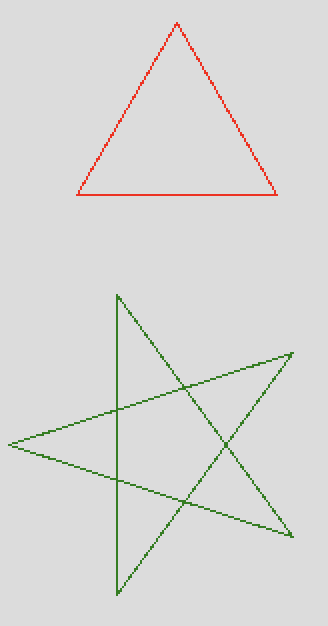
\includegraphics[width=\textwidth]{../images/turtle0.png}

\end{minipage}

\end{footnotesize}
\end{frame}

\subsection*{Konklusion}
\begin{frame}[fragile]
  \headsp{Konklusion}

  \vspace{3mm}
  \tableofcontents
\end{frame}

\end{document}
